\documentclass[slidestop]{beamer}
\usetheme{JuanLesPins}
\usepackage{fontenc}

\usepackage[english]{babel}
\usepackage[latin1]{inputenc}
\usepackage{times}
\usepackage[T1]{fontenc}
\usepackage{fontenc}
\usepackage{amssymb}
%\usepackage{pgf,pgfarrows,pgfnodes,pgfautomata,pgfheaps}
\usepackage{amsmath,amssymb}
%\usepackage{tikz}
\usepackage{times}
\usepackage{colortbl}


\title{ECB\_AT91 Libre. SBC Colombiana con soporte al sistema operativo GNU/Linux.}
\author{Carlos Iv�n Camargo Bare�o}
\institute[Universidad Nacional de Colombia]{Universidad Nacional de Colombia\\
  Departamento de Ingenier�a El�ctrica y Electr�nica\\
  EmQbit Ltda.}
\date{}

%\pgfdeclareimage[height=.5cm]{logo}{logo_unal}
%\logo{\pgfuseimage{logo}}



\begin{document}

%----------------------------------------------------------------------INSERT TITLE-
\frame[c]{\titlepage}
\frame[c]{\tableofcontents}

%$$$$$$$$$$$$$$$$$$$$$$$$$$$$$$$$$$$$$$$$$$$$$$$$$$$$$$$$$$$$$$$$$$$$$$$$$$$$$$$$$$$
%----------------------------------------------------------------------Introducci�n-
\section{Sistemas Embebidos}
%$$$$$$$$$$$$$$$$$$$$$$$$$$$$$$$$$$$$$$$$$$$$$$$$$$$$$$$$$$$$$$$$$$$$$$$$$$$$$$$$$$$

\subsection[Embedded]{Definici�n}

\begin{frame}
  \tableofcontents[current]
\end{frame}



\begin{frame}
  \frametitle{Sistemas Embebidos}\only<1>{
     \begin{block}{Definici�n}
      Los sistemas Embebidos (ES) se definen informalmente
      como ''Una Colecci�n de partes programables rodeadas 
      por ASICs y otros componentes est�ndar que interact�an 
      con un entorno a trav�s de sensores y actuadores''.
     \end{block}}
\end{frame}


\subsection{Caracter�sticas}
\frame[c]
{
\frametitle{Sistemas Embebidos - Caracter�sticas}
    \only<1,2>{
      \begin{center}
%        \includegraphics[height=3.5cm]{./images/ES_APPS.jpg}
%        \includegraphics[height=3.5cm]{./img/ES_APPS.jpg}
      \end{center}
    }
    
    \only<3>{
      \begin{center}
        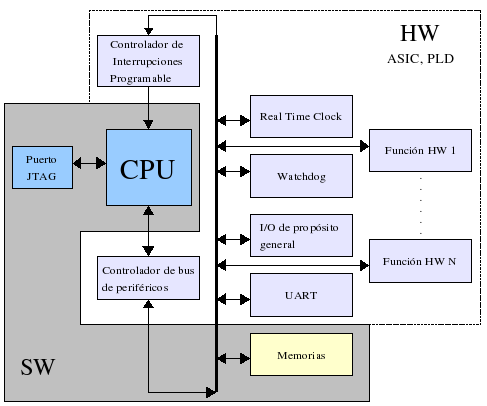
\includegraphics[height=3.5cm]{ES_Architecture}
      \end{center}
    }
    
    \only<4>{
      \begin{center}
        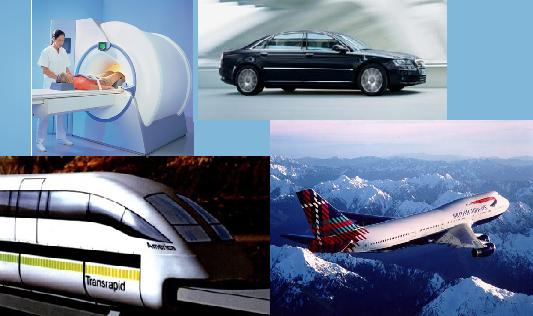
\includegraphics[height=3.5cm]{safety_ES}
      \end{center}
    }    
      
    \onslide+<1->\begin{alertblock}{Propiedades}<1->
      \begin{itemize}
        \item<1-> Dise�ados para una aplicaci�n espec�fica.
	\item<2-> Poseen (fuertes) restricciones temporales.
	\item<3-> Sistemas heterog�neos.
	\item<4-> Grandes requerimientos en t�rminos de confiabilidad.
      \end{itemize}
    \end{alertblock}
%  \end{column}
% \end{columns}
}


\subsection{Aplicaciones}

\begin{frame}
  \frametitle{Flujo de Dise�o SW en los Sistemas Embebidos}
  \begin{center}\includegraphics[scale=.30]{apps}\end{center}
\end{frame}


%$$$$$$$$$$$$$$$$$$$$$$$$$$$$$$$$$$$$$$$$$$$$$$$$$$$$$$$$$$$$$$$$$$$$$$$$$$$$$$$$$$$
%-------------------------------------------------------------Herramientas GNU     -
\section{Herramientas GNU para el desarrollo de Sistemas Embebidos}
%$$$$$$$$$$$$$$$$$$$$$$$$$$$$$$$$$$$$$$$$$$$$$$$$$$$$$$$$$$$$$$$$$$$$$$$$$$$$$$$$$$$


\begin{frame}
  \tableofcontents[current]
\end{frame}


\begin{frame}
  \frametitle{Flujo de Dise�o SW en los Sistemas Embebidos}
  \begin{center}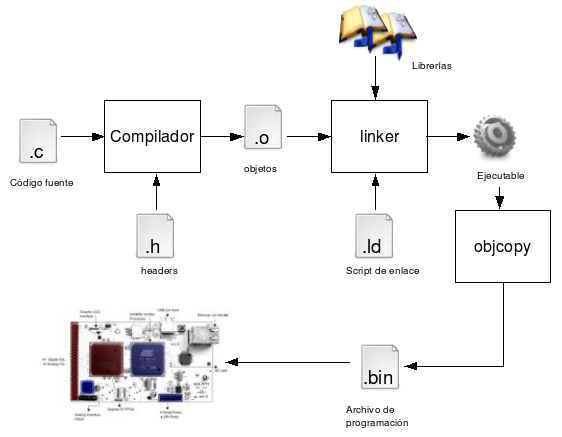
\includegraphics[scale=.40]{SW_design_flow}\end{center}
\end{frame}


\begin{frame}
  \frametitle{Algunas herramientas GNU usadas en Sistemas Embebidos}
     \begin{itemize}
	\item loader 
	\item u-boot
	\item gbibc / uclibc
	\item Linux kernel
	\item busybox / GNU fileutils, shellutils and textutils
	\item dropbear / openssh
	\item boa 
	\item sablevm
    \end{itemize}
\end{frame}

%$$$$$$$$$$$$$$$$$$$$$$$$$$$$$$$$$$$$$$$$$$$$$$$$$$$$$$$$$$$$$$$$$$$$$$$$$$$$$$$$$$$
%----------------------------------------------------------------- SBC ECB AT91    -
\section{Sistema de Desarrollo GNU Linux ECB\_AT91 }
%$$$$$$$$$$$$$$$$$$$$$$$$$$$$$$$$$$$$$$$$$$$$$$$$$$$$$$$$$$$$$$$$$$$$$$$$$$$$$$$$$$$

\begin{frame}
  \tableofcontents[current]
\end{frame}

\begin{frame}
  \frametitle{Primer SBC Colombiano ECB\_AT91}
  \begin{center}\includegraphics[scale=.30]{ECB_AT91_FREE}\end{center}
\end{frame}

\begin{frame}
  \frametitle{ECB\_AT91: Especificaciones}
  \begin{center}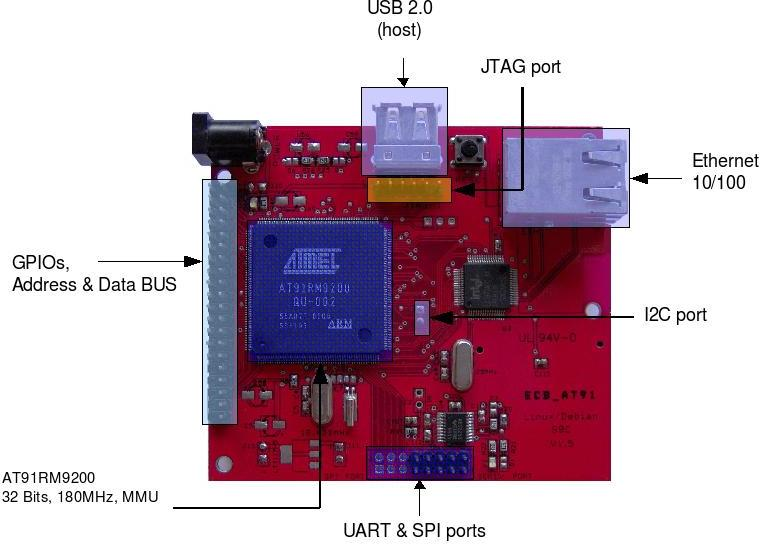
\includegraphics[scale=.90]{ECB_AT91_FREE_spec_top}\end{center}
\end{frame}

\begin{frame}
  \frametitle{ECB\_AT91: Especificaciones}
  \begin{center}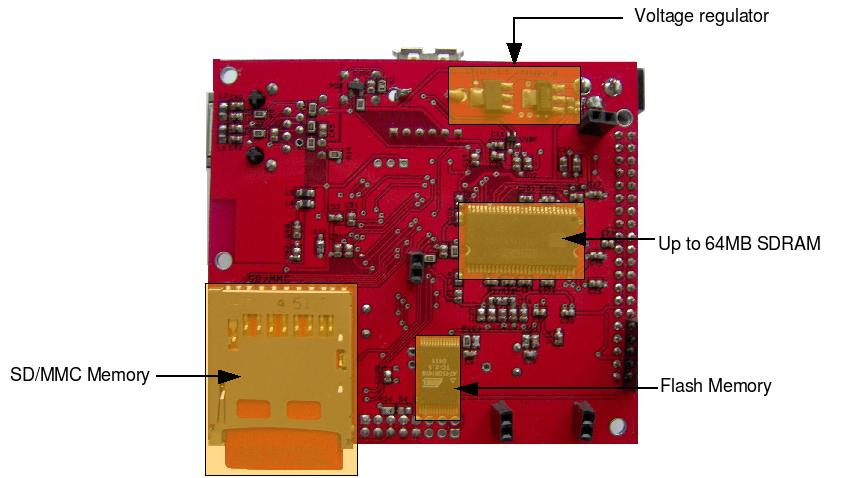
\includegraphics[scale=.30]{ECB_AT91_FREE_spec_bot}\end{center}
\end{frame}

\begin{frame}
  \frametitle{SBC En acci�n}
  \begin{center}\includegraphics[scale=.30]{ECB_AT91_TUX}\end{center}
\end{frame}

\begin{frame}
  \frametitle{Enlaces}
  
  P�gina de la ECB\_AT91 Libre
  \begin{itemize}
  \item
    \url{http://wiki.emqbit.com/free-ecb-at91}
  \end{itemize}
  
  P�gina del grupo de trabajo sobre GNU Linux en sistemas embebidos
  \begin{itemize}
  \item
    \url{http://wiki.freaks-unidos.net/linuxencaja}
  \end{itemize}
\end{frame}


\begin{frame}
  \begin{center}
\includegraphics[scale=.15]{gracias}
  \newline
  \huge{�Gracias!}
  \end{center}
\end{frame}

\end{document}
